\chapter{Result}
Här är väl tanken att jag ska skriva lite om hur jag implementerat
och bearbetat allt relevant som har med implementationen att göra. 
Vad jag gjort som blivit bättre än andra lösningar. Vad jag fokuserat
på (throughput kontra mängd använd hårdvara).

\section{Problems}
Encountered problems:

\begin{itemize}
\item Not possible to get the license for CSA3
\item Small interrest for CSA3
\item Next to no documentation of the CISSA algorithm
\end{itemize}

% Fortsätt fylla i när du stöter på problem

\section{Hardware}
Såhär ser hårdvaran ut i en sjukt snygg bild jag ritat: \newline

\begin{array}{r l c r l}
  Inputs & &  \_\_\_\_\_\_\_ & & Outputs \\
  1 & --| & & | -- & 1 \\
  2 & --| & & | -- & 2 \\
  3 & --| & HW & | -- & 3 \\
  4 & --| & & | -- & 4 \\
  5 & --| & & | -- & 5 \\
  &     &   \_\_\_\_\_\_\_ & & \\
\end{array}

\section{Flow}
Berätta om flödet på implementationen.

\section{Special solutions}
Berätta om hur det fungerar.

\section{Implementation}
My design is very hierarchical. The top layer is an aes128 block in CBC-mode. 
It takes an input TS-stream, scrambles it, and outputs a TS-stream. 

\subsection{CBC entity}
\Warning[Write this]{when you have started implementing the cbc mode of aes 
  encryption}
The CBC entity consists of ??!??! entities. It is responsible for looking for an 
adaptation field in the header, since the amount of and placement of data depends
on if it exists or not. There is only going to be one aes128 cipher block 
implemented, instead of running all of the TS-packets in parallell, they are to 
be scrambled in sequence to decrease the amount of hardware usage.

\subsection{Cipher entities}
The aes-128 cipher entity consists of 4 components. The data2state entity, which 
transforms the array into a matrix of data. A keyexpansion entity, which takes 
an input of a key, and generates an extended key as an output. An entity, which I
chose to call rounds, which deals with the encryption of the 16 byte blocks. And 
finally a state2data entity, which transforms the data-matrix into an array once 
again. The cipher entity itself keeps track of timing mainly between the 
keyexpansion and the round entity, and makes sure to provide the round entity 
with the correct roundkey at the right time.

\subsection{Keyexpansion entities}
The keyexpansion entity is divided into 3 keyblock entities. The first keyblock 
entity decides what 4 bytes of the expanded key we want to expand. The second 
keyblock entity is the keycore, which is only performed on every 4th set of 
4 bytes. The third keyblock entity performs an xor and an incrementation of the 
internal counter used as an index when accessing 4 byte blocks of data.

\subsubsection{Keycore entitites}
The keycore entity consists of four entities. Rotword, Sbox, Rcon and a counter. 
The counter is used to get the right data-byte from the Rcon, and the index is 
only used in the keycore, and is thus best suited to be placed inside the 
keycore entity. Rotword rotates the bytes of the input one step to the left. 
Sbox replaces the input bytes according to the Rijndael Sbox. The Rcon entity 
both collects the correct rcon value from a precalculated vector, as well as 
inputs it into an xor together with the input.

\subsection{Round entities}
The round block consists of four entities. Subbytes, shiftrows, mixcolumns and 
addroundkey. Addroundkey is a somewhat special XOR. Subbytes is an Rijndael 
Sbox, which takes an input 16-byte state, substitutes it, and outputs another 
16-byte state. Shiftrows transposes the rows of the second, third and fourth 
row of the state. Last, but not least, is the mixcolumns entity. It consists of 
16 mulblock entities. The input state of mixcolumns is split into columns, and 
each column is sent to a mulblock entity, which multiplies the inputs according 
to an amount of rules. The function of the mixcolumns block is a rather complex 
matrix multiplication.

\subsubsection{Addroundkey entity}
Addroundkey is an entity which takes different inputs depending on 
what round we are currently dealing with. On the first round, addroundkey takes 
the input to the round entity. On the last round, it takes the output from the 
subbytes entity. The input to addroundkey is the output from mixcolumns the rest 
of the time.

\subsubsection{The mulblock entity}
The mulblock entity consists of one mul3 entity and one mul2 entity, which 
performs a special kind of hardware multiplication of 3, and 2, on the input. It 
also takes two inputs which it leaves alone. The four results are then XOR:ed 
with eachother, and returned to the mixcolumns entity which puts the result in 
the correct index in the matrix.

\section{Tests}
\Warning[omformulera]{Är det här för casual? Du måste nog omformulera varför du 
  inte lagt till fler simuleringsresultat}
I simulated all of the subblocks I have written, one by one, to make sure that 
they had the correct functionality Even though I've only input a few simulations 
in this part. The reason why not more simulations are included is mainly since 
I do not think anyone will find it interresting enough to look through, and since
I do not want to double the volume of the thesis through simulation results.

Figure \ref{test:1} through \ref{test:3} are tests performed on the complete 
aes-128 block, before CBC-mode. In the figures, in\_key is the input key to be 
extended and used, and datapacket is one packet from a TS. Test vector 1 and 2 
are taken from \citep{AES:2001}, while test vector 3 is generated using a 
webpage.

\emph{Test vector 1 (Figure \ref{test:1})}\\
Input key: 2b 7e 15 16 28 ae d2 a6 ab f7 15 88 09 cf 4f 3c\\
Plaintext: 32 43 f6 a8 88 5a 30 8d 31 31 98 a2 e0 37 07 34\\
Ciphertext: 39 25 84 1d 02 dc 09 fb dc 11 85 97 19 6a 0b 32

\begin{figure}
  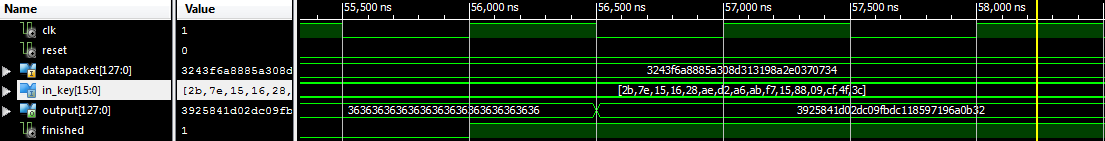
\includegraphics[width=\textwidth]{successtv1}
  \caption{Test vector 1}
  \label{test:1}
\end{figure}

\emph{Test vector 2 (Figure \ref{test:2})}\\
Input key: 00 01 02 03 04 05 06 07 08 09 0a 0b 0c 0d 0e 0f\\
Plaintext: 00 11 22 33 44 55 66 77 88 99 aa bb cc dd ee ff\\
Ciphertext: 69 c4 e0 d8 6a 7b 04 30 d8 cd b7 80 70 b4 c5 5a

\begin{figure}
  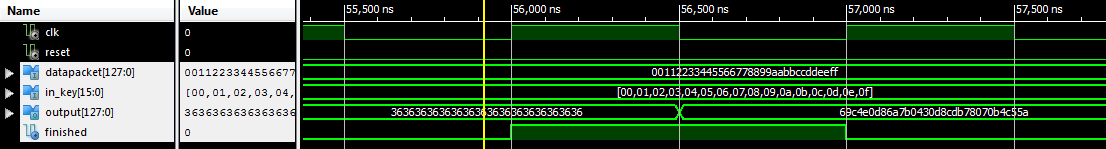
\includegraphics[width=\textwidth]{successtv2}
  \caption{Test vector 2}
  \label{test:2}
\end{figure}

\emph{Test vector 3 (Figure \ref{test:3})} \\
Input key: 10 20 30 40 50 60 70 80 90 a0 b0 c0 d0 e0 f0 bb\\
Plaintext: 00 11 22 33 44 55 66 77 88 99 aa bb cc dd ee ff\\
Ciphertext: bf 99 1f aa 8b 0f e6 48 36 46 a0 2d 33 9e de a5

\begin{figure}
  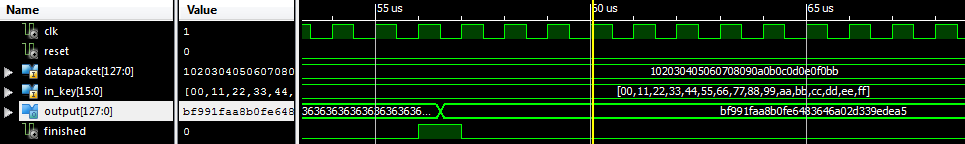
\includegraphics[width=\textwidth]{successtv3}
  \caption{Test vector 3}
  \label{test:3}
\end{figure}
